\section{The Polynomial-time Hierarchy}
    \subsection{Basic definitions and properties}
        \begin{frame}{Definitions}
            \begin{block}{Definition: $\Sigma_k^P$}
                $ \Sigma_0^P := P$\\
                For $k\geq 1:$ \\
                $L \in \Sigma_k^P \iff $ there are polynomials $p_1, p_2,..., p_k$ and a polynomial-time predicate $F$ s.t.:
                $$x \in L \leftrightarrow 
                    \existss{y_1 \in S_1\text{ }}{}
                    \foralll{y_2 \in S_2\text{ }}{}
                    \exists ...\underset{y_k \in S_k}{Q} F(x,y_1,...,y_k)$$
                where $S_i := \{0,1\}^{p_i(|x|)}$  
            \end{block}
        \end{frame}
        \begin{frame}{Definitions}
            \begin{block}{Definition: $\Pi_k^P$}
                $ \Pi_0^P := P$\\
                For $k\geq 1:$ \\
                $L \in \Pi_k^P \iff $ there are polynomials $p_1, p_2,..., p_k$ and a polynomial-time predicate $F$ s.t.:
                $$x \in L \leftrightarrow 
                    \foralll{y_1 \in S_1\text{ }}{}
                    \existss{y_2 \in S_2\text{ }}{}
                    \forall ...\underset{y_k \in S_k}{Q} F(x,y_1,...,y_k)$$
                where $S_i := \{0,1\}^{p_i(|x|)}$  
            \end{block}
        \end{frame}

        \begin{frame}{Definitions}
            \begin{block}{Definition: The Polynomial-time Hierarchy $PH$}
            $PH := \bigcup\limits_{i \in \mathbb{N}} \Sigma_i^P \cup \Pi_i^P $
            \end{block}
        \end{frame}
    
        \begin{frame}{Structural Properties}  
            for all $i\in \mathbb{N}$: 
            \begin{enumerate}
                \item $\Pi_i^P = co\Sigma_i^P $
                \pause
                \item $\Sigma_i^P \subseteq \Sigma_{i+1}^P \cap \Pi_{i+1}^P$
                \item $\Pi_i^P \subseteq \Sigma_{i+1}^P \cap \Pi_{i+1}^P$
                \pause
                \item (?)$\Sigma_i^P \subset \Sigma_{i+1}^P$
            \end{enumerate}
        \end{frame}

        \begin{frame}{Scheme of the Polynomial-time hierarchy}            
            \begin{figure}
                \centering
                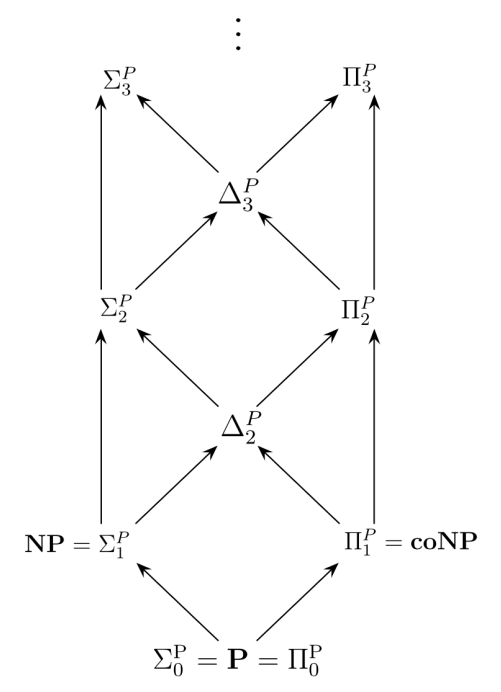
\includegraphics[scale=.4]{images/PH.png}
                \caption{The Polynomial-time Hierarchy.}
                \label{fig:The Polynomial-time Hierarchy}
            \end{figure}
        \end{frame}

        \begin{frame}{Equivalent definition}
            \begin{block}{lemma}
                For all $k, L \in  \Sigma_{k+1}^P \iff $
                there is a polynomial $p$ and $A \in \Pi_k^P$:
                $$x \in L \leftrightarrow 
                \existss{y\in \{0,1\}^{p(|x|)}}{} <x,y> \in A$$
            \end{block}
            \pause
            \begin{block}{Proof$(\Leftarrow)$}
                $<x,y> \in A \leftrightarrow \foralll{y_1 \in S_1\text{ }}{}
                    \existss{y_2 \in S_2\text{ }}{}
                    \forall ...\underset{y_k \in S_k}{Q} F(<x,y>,y_1,...,y_k)$\\
                for some polynomial F and $S_i := \{0,1\}^{p(|x|)_i}$ for polynomials $p_1,p_2,..., p_k$
                . Putting this in the equation gives us the desired result in one direction.
            \end{block}
        \end{frame}

        \begin{frame}{Equivalent definition}
            \begin{block}{Proof$(\Rightarrow)$}
                $$x \in L \leftrightarrow 
                \existss{y \in S\ }{}
                \foralll{y_1 \in S_1\ }{}
                \exists ...\underset{y_k \in S_k}{Q} F(x,y,y_1,...,y_k)$$
                Where, $S:= \{0,1\}^{p(|x|)}$ and $S_i$ as before for 
                $i= 1 ,... ,k$. \\
                Let $$\hat{p}(n):= n^{deg(p)+1}+M $$ 
                for a large enough $M$ such that
                $\forall n\ \hat{p}(n) \geq p(n)$.
            \end{block}
        \end{frame}

        \begin{frame}{Equivalent definition}
            \begin{block}{Proof$(\Rightarrow)$}
                Now define:\\
                $\hat{F}(z,y_1,...y_k)$
                \begin{algorithmic}[1]
                    \State $L := min\{t|\hat{p}(t)+t=|z|\}$
                    \If {$L = None$}
                        \State return False
                    \EndIf
                    \State return $F(z[1,..,L],z[L+1,...,L+p(L)],y_1,...y_k)$
                \end{algorithmic}
                Then we have this nice property:
                \begin{align*}
                x \in L  
                & \leftrightarrow 
                \existss{y \in S\ }{}
                \foralll{y_1 \in S_1\ }{}
                \exists ...\underset{y_k \in S_k}{Q} F(x,y,y_1,...,y_k) \\
                & \leftrightarrow
                \existss{\hat{y} \in {\{0,1\}}^{\hat{p}(x)}\ }{}
                \foralll{y_1 \in S_1\ }{}
                \exists ...\underset{y_k \in S_k}{Q} 
                \hat{F}(<x,\hat{y}>,y_1,...,y_k)
                \end{align*}
            \end{block}
        \end{frame}

        \begin{frame}{Equivalent definition}
            \begin{block}{Proof$(\Rightarrow)$}
                Now put:\\
                $$ A:= \{z| 
                \foralll{y_1 \in S_1\ }{}
                \exists ...\underset{y_k \in S_k}{Q} 
                \hat{F}(z,y_1,...,y_k)\} $$
                But $\hat{F}$ is clearly polynomial-time, which means
                $A \in \Pi_k^P$.
                Finally:
                \begin{align*}
                    x \in L  
                    & \leftrightarrow
                    \existss{\hat{y} \in {\{0,1\}}^{\hat{p}(x)}\ }{}
                    \foralll{y_1 \in S_1\ }{}
                    \exists ...\underset{y_k \in S_k}{Q} 
                    \hat{F}(<x,\hat{y}>,y_1,...,y_k)\\
                    & \leftrightarrow
                    \existss{y\in \{0,1\}^{\hat{p}(|x|)}}{} <x,y> \in A
                    \end{align*}
                this completes the proof.
            \end{block}
        \end{frame}
            
        \begin{frame}{Collapsibility}
            \begin{block}{lemma}
                For all $k, L \in  \Pi_{k+1}^P \iff $
                there is a polynomial $p$ and $A \in \Sigma_k^P$:
                $$x \in L \leftrightarrow 
                \foralll{y\in \{0,1\}^{p(|x|)}}{} <x,y> \in A$$
            \end{block}
            \pause
            \begin{block}{Theorem: PH is collapsible}            
                $i \geq 1 $ \& $ \Pi_i^P = \Sigma_i^P \to PH = \Sigma_i^P$
            \end{block}
        \end{frame}

        \begin{frame}{Collapsibility}
            \begin{proof}
                \small{
                It suffices to show that 
                $i\geq1 \text{ $\&$ } \Sigma_i^P = \Pi_i^P 
                \to \Sigma_i^P = \Sigma_{i+1}^P$:\\
                $L \in \Sigma_{i+1}^P \iff$ there is a polynomial $p$ and $A \in \Pi_i^P$:
                $$x \in L \leftrightarrow \existss{|y|=p(|x|)}{} <x,y> \in A$$
                $\iff$ there are $A \in \Sigma_i^P$ and $p$:
                 $...$\\
                $\iff$ there are $p,p'$ and $B \in \Pi_{i-1}^P$:
                $$x \in L \leftrightarrow \existss{|y|=p(|x|)}{} \existss{|y'|=p'(|x|)}{} <x,y,y'> \in B$$
                $\iff$ there are $p'' = p+p'$ and $B \in \Pi_{i-1}^P$:
                $$x \in L \leftrightarrow \existss{|y''|=p"(|x|)}{} <x,y''> \in B$$
                $\iff L \in \Sigma_i^P$.
                }
            \end{proof}
        \end{frame}

    \subsection{Relationships to other  complexity classes}
        \begin{frame}{Relationships to other complexity classes}  
            \begin{block}{Review: NP}
                $L \in NP \iff $ there is a polynomial $p$ and a polynomial-time predicate $F$ s.t.:
                $$x \in L \iff \existss{|y| \leq p(|x|)}{} F(x,y)$$
            \end{block}
            \pause
            \begin{block}{Lemma}
                $NP = \Sigma_1^P$
            \end{block}
            \pause
            \begin{block}{Proof}
                \begin{enumerate}
                    \item  for one direction use padding to fix the length of y
                    \item for the other direction check the length of y in algorithm
                \end{enumerate}                
            \end{block}
        \end{frame}
        
        \begin{frame}{Relationships to other  complexity classes} 
            \begin{block}{Definition: BPP}
                $L \in BPP \iff $ there is a polynomial $p$ and a polynomial-time randomized algorithm $F$ s.t.:
                $$x \in L \implies \underset{r\in \{0,1\}^{p(|x|)}}{Pr}(F(x,r)) \geq 2/3$$
                $$x \notin L \implies \underset{r\in \{0,1\}^{p(|x|)}}{Pr}\ (F(x,r)) \leq 1/3$$
            \end{block}
            \begin{table}
                \centering
                \begin{tabular}{rcc}
                     & $F(x,r)$ & $\neg F(x,r)$ \\\hline
                    $x \in L$ & \(\geq 2/3\) & \(\leq 1/3\) \\
                    $x \notin L$ & \(\leq 1/3\) & \(\geq 2/3\) \\
                \end{tabular}
                \caption{$\underset{r\in \{0,1\}^{p(|x|)}}{Pr}\ (F(x,r))$}
                \label{BPP DEF}
            \end{table}
        \end{frame}

        \begin{frame}{Relationships to other complexity classes}
            \begin{block}{lemma}
                $BPP$ is closed under complement.
            \end{block}
            \begin{block}{Proof.}
                Immediate from definition.
            \end{block}
        \end{frame}

        \begin{frame}{Relationships to other complexity classes}
            \begin{block}{lemma}
                If $L \in BPP$ then there is an algorithm $F$ such that:
                $$\forall x \ 
                    \underset{r}{Pr}\ (F(x,r) = right\ answer) 
                    \geq 1-\frac{1}{3|x|}$$
            \end{block}
        \end{frame}

        \begin{frame}{Relationships to other complexity classes}
            \begin{block}{Proof.}
                Since $L \in BPP$ then there is a polynomial-time two-sided 
                Monte Carlo algorithm $A$, which gives the right answer
                with probability at least $\frac{1}{2}+\epsilon$ for some 
                $ 0 < \epsilon \leq \frac{1}{2}$. Now recall the algorithm 
                $A_t$ from the book, which repeats $A$ for $t$ times and 
                output a solution if $A$ outputs that solution for at least
                $\lceil \frac{t}{2} \rceil$ times. As it is shown in the
                book, it is enough to set $t \geq 
                \frac{2ln \frac{2}{3|x|}}{ln(1-4 \epsilon^2)}$
                 to have that
                $$ \underset{r}{Pr}\ (A_t(x,r) = right\ answer) 
                    \geq 1-\frac{1}{3|x|}$$
            \end{block}
        \end{frame}

        \begin{frame}{Relationships to other complexity classes}
            \begin{block}{Proof.}
                This means that instead of a fixed $t$ in $A_t$, it's enough 
                that the algorithm calculates the proper $t$ as above, and then 
                continues. Clearly this calculation takes place in polynomial-
                time. On the other hand it's enough to have 
                $t \in O(|ln\frac{2}{3|x|}|) = O(ln(|x|))$, and 
                since $A$ runs in polynomial-time, then repeating $A$ for 
                $O(ln(|x|))$ is again a polynomial-time task. This completes
                the proof.
            \end{block}
        \end{frame}

        \begin{frame}{Relationships to other complexity classes}
            \begin{block}{Theorem}
                $BPP \subseteq \Sigma_2$
            \end{block}
            \pause
            \begin{block}{Proof.}
                Let $L \in BPP$ and $F$ has the property in the previous
                lemma and let $ m = |x|$. We show the following:
                $$x\in L \iff \exists y_1,y_2,...,y_{m} \in {\{0,1\}}^{m}
                \forall z \in {\{0,1\}}^{m} \orr{i=1}{m} F(x,y_i\oplus z)$$
            \end{block}
        \end{frame}

        \begin{frame}{Relationships to other complexity classes}
            \begin{block}{Proof.}
                $\Rightarrow$: Suppose $x \in L$, then 
                \begin{align*}
                    & \underset{y_1,y_2,...,y_m}{Pr}\ 
                    (\forall z \in {\{0,1\}}^m 
                     \orr{i=1}{m} F(x,y_i\oplus z))\\
                    & = 1- \underset{y_1,y_2,...,y_m}{Pr}\ 
                    ( \exists z \in {\{0,1\}}^m
                     \andd{i=1}{m} \neg F(x,y_i\oplus z))\\
                    & \geq 1- \sum\limits_{z\in{\{0,1\}}^{m}} 
                    \underset{y_1,y_2,...,y_m}{Pr}\ 
                    (\andd{i=1}{m} \neg F(x,y_i\oplus z))\\
                    & \geq 1-  \frac{2^{m}}{{(3m)}^{m}} > 0.
                \end{align*}
            This implies that there are $y_1,y_2,...,y_m$ such that:
            $$\forall z \in {\{0,1\}}^{m} \orr{i=1}{m} F(x,y_i\oplus z)$$
            \end{block}
        \end{frame}

        \begin{frame}{Relationships to other complexity classes}
            \begin{proof}
                $\Leftarrow$: Suppose $x \notin L$, then for an arbitrary
                sequence $y_1,...y_m \in {\{0,1\}}^{m}$
                \begin{align*}
                    \underset{z}{Pr} \
                    (\andd{i=1}{m} \neg F(x,y_i\oplus z))
                    & = 1 -\underset{z}{Pr}\ 
                        (\orr{i=1}{m} F(x,y_i\oplus z)) \\
                    & \geq 1- \sum\limits_{i=1}^m
                     \underset{z}{Pr}\ 
                     (F(x,y_i\oplus z)) \\
                    & \geq 1-  \frac{m}{3m} >0.
                \end{align*}
                Thus:
                $$\forall y_1,...,y_m \exists z \in {\{0,1\}}^m
                    \neg \orr{i=1}{m} F(x,y_i\oplus z)) $$
            \end{proof}
        \end{frame}
                
        \begin{frame}{Relationships to other complexity classes}
            \begin{block}{Sipser–Lautemann theorem}
                $BPP \subseteq \Sigma_2^P \cap \Pi_2^P$
            \end{block}
            \begin{block}{Proof.}
                Use the previous lemma and the fact that $BPP$ is closed
                under complement.
            \end{block}
        \end{frame}

        \begin{frame}{Relationships to other  complexity classes}
            \begin{block}{Theorem}
                $PH \subseteq PSPACE$
            \end{block}
        \end{frame}

        \begin{frame}{Relationships to other  complexity classes}
            \begin{block}{Proof}
                It is sufficient to show that for any $i$ if $\Pi_i \subseteq PSPACE$ then $\Sigma_{i+1} \subseteq PSPACE$:\\
                Suppose $L \in \Sigma_{i+1}$ then there is a polynomial $p$ and $A \in \Pi_i^P$:
                $$x \in L \leftrightarrow \existss{y\in \{0,1\}^{p(|x|)}}{} <x,y> \in A$$
                $A$ is decidable in $PSPACE$ by hypothesis, 
                thus $\existss{y\in \{0,1\}^{p(|x|)}}{} <x,y> \in A$
                 is decidable in $PSPACE$ using the odometer method.
            \end{block}
        \end{frame}

        \begin{frame}{Relationships to other  complexity classes}
            \begin{block}{Lemma}
                For all $i$: $\Sigma_i^P$  is closed under $\leq_p$
            \end{block}
            \pause
            \begin{block}{Proof}
                $A \leq_p B \iff$ there is a polynomial algorithm $R$:
                    $$x\in A \iff R(x) \in B$$
                Now suppose $B \in \Sigma_i^P$ then:
                $$x \in A \leftrightarrow 
                    \existss{y_1 \in S_1\text{ }}{}
                    \foralll{y_2 \in S_2\text{ }}{}
                    \exists ...\underset{y_k \in S_k}{Q} F(R(x),y_1,...,y_k)$$
                where $S_i := \{0,1\}^{p_i(|R(x)|)}$
            \end{block}
        \end{frame}
        \begin{frame}{Relationships to other  complexity classes}
            \begin{block}{Theorem}
                $PH = PSPACE \implies PH$ Collapses.
            \end{block}
            \pause
            \begin{block}{Proof}
                $PH = PSPACE \implies PH$ have a complete problem which is in $\Sigma_i$ for some $i$ and since $\Sigma_i$ is closed under $\leq_p$: $\Sigma_i = PH$
            \end{block}
        \end{frame}
        
        \begin{frame}{Relationships to other  complexity classes}   
            \begin{enumerate}
                \item $NP = \Sigma_1^P $ $\&$ $ CoNP = \Pi_1^P$
                \pause
                \item $P = NP \iff P = PH$
                \pause
                \item $BPP \subseteq \Sigma_2^P \cap \Pi_2^P $
                \pause
                \item $PH \subseteq PSPACE$
                \pause
                \item $PH = PSPACE \implies PH$ Collapses.
            \end{enumerate}
        \end{frame}
        
        \begin{frame}{Complexity classes}            
            \begin{figure}
                \centering
                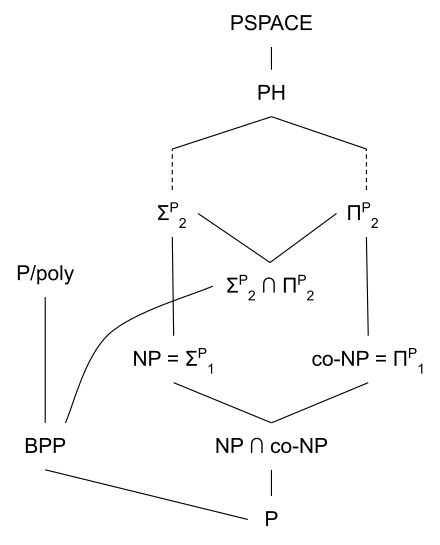
\includegraphics[scale=0.5]{images/PH2.png}
                \caption{Complexity Classes Inclusion Tree}
                \label{fig:focuslogo}
            \end{figure}
        \end{frame}